\documentclass{article}

% if you need to pass options to natbib, use, e.g.:
%     \PassOptionsToPackage{numbers, compress}{natbib}
% before loading neurips_2021

% ready for submission
% \usepackage{neurips_2021}

% to compile a preprint version, e.g., for submission to arXiv, add add the
% [preprint] option:
% \usepackage[preprint]{neurips_2021}

% to compile a camera-ready version, add the [final] option, e.g.:
%     \usepackage[final]{neurips_2021}

% to avoid loading the natbib package, add option nonatbib:
\usepackage[nonatbib,preprint]{neurips_2021}

\usepackage[utf8]{inputenc} % allow utf-8 input
\usepackage[T1]{fontenc}    % use 8-bit T1 fonts
\usepackage{hyperref}       % hyperlinks
\usepackage{url}            % simple URL typesetting
\usepackage{booktabs}       % professional-quality tables
\usepackage{amsfonts}       % blackboard math symbols
\usepackage{nicefrac}       % compact symbols for 1/2, etc.
\usepackage{microtype}      % microtypography
\usepackage{xcolor}         % colors
\usepackage{graphicx}
\usepackage[numbers]{natbib}

\title{Final Paper: A Framework for Leveraging Small Language Models for Synthetic Data Generation for
Fine-Tuning}

% The \author macro works with any number of authors. There are two commands
% used to separate the names and addresses of multiple authors: \And and \AND.
%
% Using \And between authors leaves it to LaTeX to determine where to break the
% lines. Using \AND forces a line break at that point. So, if LaTeX puts 3 of 4
% authors names on the first line, and the last on the second line, try using
% \AND instead of \And before the third author name.

\author{%
  Zachary Grannan \\
  \And{}
  Owen Ren
}

\begin{document}

\maketitle

\begin{abstract}
Synthetic data is now commonly used in LLM post-training. However, there has
been less research into the use of domain-specific synthetic data for
fine-tuning purpose-built LLMs. We propose the development of an open-source
agentic framework, in the style of AgentInstruct
\citep{mitra_agentinstruct_2024}, to automatically generate synthetic data for
domain-specific LLM fine-tuning. We will come the performance of LLMs fine-tuned
via our framework to traditional RAG-based approaches.
\end{abstract}

\section{Introduction}
Many commercial applications of large language models (LLMs) involve applying them to solve domain-specific tasks. Often, such applications require that additional domain-specific information, in particular information outside of the LLM training data, is made available to the LLM.

Retrieval-augmented generation (RAG) \citep{lewis_retrieval-augmented_2020} is a
popular technique for making such information available. In RAG, the application
injects data (e.g. from a database) into the system prompt, with the hope that
the LLM can use this information to produce a response that incorporates
relevant domain-specific data. An advantage of the RAG-based approach is its
flexibility and ease-of-use: the application can use its own logic to determine
how to enhance the prompts. However, RAG systems have corresponding
disadvantages. In particular, incorporating a RAG architecture increases
application and infrastructure complexity.

Fine-tuning presents another approach. In the fine-tuning paradigm, the parameters of the LLM itself are modified by training the LLM on additional content. The fine-tuned LLM can be used as a "drop-in" replacement for a base language model: no changes to architecture or software are required.

In prior work, various recipes have been proposed for developing specialized LLMs via fine-tuning \citep{balaguer_rag_2024,yang_fingpt_2023,wu_pmc-llama_2023}. Simultaneously, various techniques have been developed to improve general reasoning abilities with synthetic data \citep{shao_synthetic_2023,wang_self-instruct_2023,mitra_agentinstruct_2024}.

However, there is relatively less literature evaluating the performance of
state-of-the-art synthetic data generation techniques for fine-tuning
domain-specific LLMs. AgentInstruct \citep{mitra_agentinstruct_2024} provides a promising
agent-based approach, however the authors did not perform any evaluation for
domains-specific cases, and the AgentInstruct code is not readily available.

For this project, we propose the development of an open-source agentic framework
(in the style of AgentInstruct) that can automatically generate synthetic data
and fine-tune an LLM on that data. Concretely, we wish to make the following
contributions:

\begin{enumerate}
\item The development of the aforementioned framework
\item An evaluation that compares the performance of LLMs fine-tuned via our framework to traditional RAG based techniques
\item Reproducible experiments that track resource usage and the ability to leverage different language models
\end{enumerate}

\section{Related Work}

With the rapid advancements of new large language models (LLMs), there is
concern that the amount of internet data that has traditionally been used to
train these models has been exhausted. Recent releases of the latest models
have used synthetic data during pre- and post-training \citep{abdin_phi-3_2024,
dubey_llama_2024, bai_qwen_2023}. Furthermore, the generative and reasoning
capabilities of LLMs have proven their effectiveness as tools for synthetic data
generation.

\subsection{Fine-Tuning with Synthetic Data}

Recent research into leveraging LLMs for synthetic data generation is split
into two approaches: seeded methods where LLMs are guided by an initial dataset
to generate new data and seedless methods where LLMs generate data without an
initial dataset. In Self-Instruct \citep{wang_self-instruct_2023}, the authors
leverage vanilla GPT-3 to generate instructions, input, and output samples to
fine-tune the same language model, demonstrating a 33\% improvement over the
original model. In Synthetic Prompting \cite{shao_synthetic_2023}, they leverage
an LLM to generate Chain-of-Thought prompts to enhance a language model’s
reasoning capabilities during inference. In TarGEN \citep{gupta2023targen}, the
authors present a seedless multi-step prompting strategy that generates
high-quality synthetic datasets using LLMs, including on domain-specific tasks
with minimal existing data. Recent approaches to using LLMs for synthetic data
generation have led to agentic approaches that generate large amounts of diverse
and high-quality data. In AgentInstruct \citep{mitra_agentinstruct_2024}, seed
data is leveraged to transform and generate new data using curated LLM agents
across 17 different skills ranging from reading comprehension, question
answering, creative writing to few-shot reasoning. The resulting fine-tuned
Orca-3 model trained on the 22 million instructions generated from AgentInstruct
outperforms GPT-3.5-turbo and GPT-4 in the MMLU and DROP benchmarks.

\subsection{Integrating Knowledge Retrieval and Fine-Tuning}

Recent literature in combining fine-tuning with RAG, RAFT \citep{zhang2024raft},
has shown improvements in performance across domain-specific datasets. REALM
\citep{guu_realm_2020} augments a language model with a neural knowledge
retrieval engine that is also trained during the pre-training and fine-tuning
stages.

\subsection{Efficient Fine-Tuning}

Advancements in both fine-tuning, in which an existing model’s weights are used
as the baseline for further training, and improvements in small language models
have drastically reduced the computation required to fine-tune a model. Methods
like LoRA \citep{hu2021lora} and QLoRA \cite{dettmers2024qlora} have further
reduced the computation requirements for LLM finetuning.

While Large Language Models have significantly advanced natural language
processing, small language models (SLM) have also seen improvements in text
generation, reasoning, and performance. Training techniques such as model
distillation use an LLM to fine-tune an SLM, transferring knowledge from the LLM
to the SLM. Furthermore, SLMs have advantages in cost, computation, and
flexibility over LLMs. While LLMs excel at generalisability, recent research has
shown that SLMs fine-tuned on domain-specific datasets can outperform
general-purpose LLMs for specific tasks.

\subsection{Domain-Specific LLMs}

Domain-specific LLMs, both those trained from scratch and those that fine-tune
an existing model, have been shown to outperform general-purpose LLMs. In the
former category, the closed-source BloombergGPT \citep{wu_bloomberggpt_2023},
trained from scratch on a dataset consisting of domain-specific and general
data, outperforms general-purpose LLMs on finance-related tasks.

Because training an LLM from scratch is extremely resource-intensive, approaches
based on fine-tuning are often more economically feasible. Such approaches
typically fine-tune an LLM by injecting additional knowledge and performing
instruction-tuning \citep{ouyang_training_2022}. FinGPT \citep{yang_fingpt_2023}
provides a framework for fine-tuning LLMs for finance-related tasks. The
lightweight model PMC-LLaMa \citep{wu_pmc-llama_2023} is developed by
fine-tuning a LLaMA model, and can outperform ChatGPT on various medical QA
tasks.

\section{Methodology}

\begin{figure}[h]
  \centering
  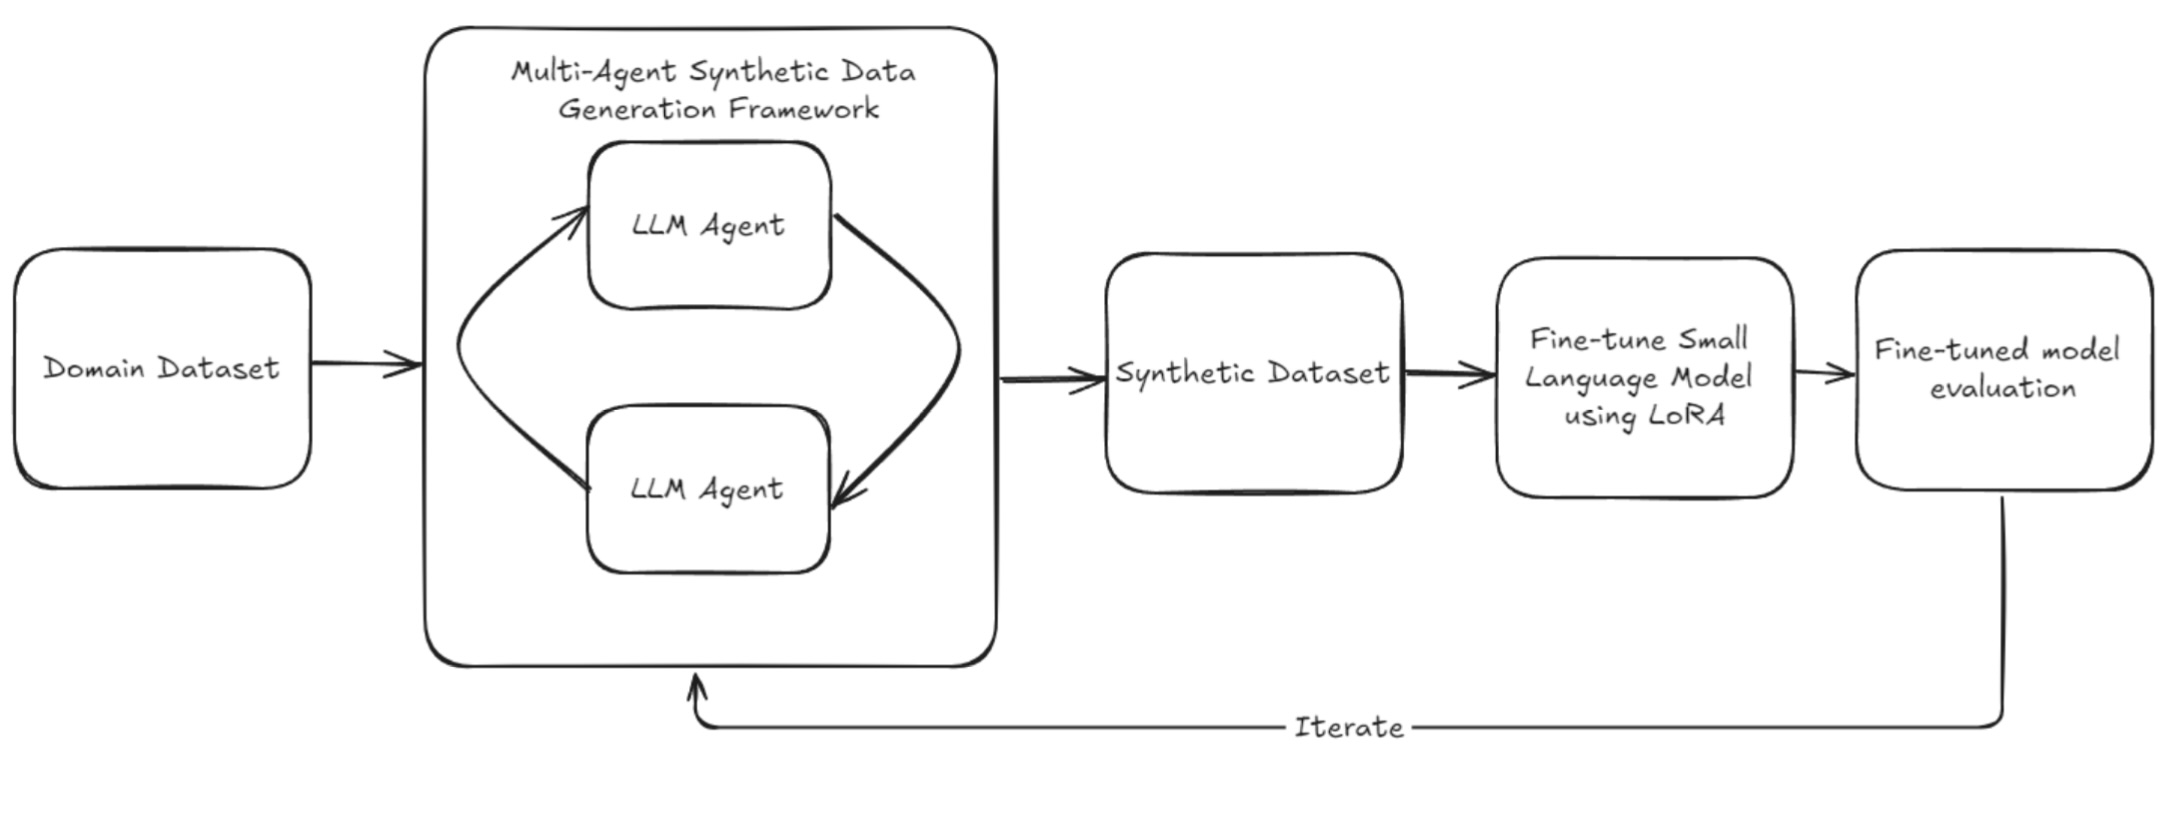
\includegraphics[width=1\textwidth]{methodology.jpg}
  \caption{An overview of our methodology. TODO}
\end{figure}

For our domain datasets that will be used as the seed data, we are still currently exploring datasets that can be used. Current ideas include research papers, company financial data, technical reports and manuals, or company specific FAQ data.
We will develop a multi agent synthetic data generation framework using small language models such as Llama-3.1-8B, Llama-3.2-3B, Qwen2.5-7B to synthetically generate high-quality diverse domain specific data.. Our immediate goal will be to create a framework for specializing in question answering tasks, similar to that of a traditional chatbot. Time permitting, we may expand this scope to also minimize hallucinations from model responses.
Next we will use the data to fine-tune LoRA adapters on the base model chosen. Since this will be an iterative process, we may also choose to perform a full supervised fine-tune of the model depending on resource limitations.

\subsection{Challenges}

One of the challenges we foresee may be overfitting on the fine-tuned model and the models inability to generalize to different writing styles and formats. We plan to mitigate this by increasing the diversity of our generated data. Another challenge is hallucination: previous research has shown that fine-tuning LLMs with new factual information increases their tendency to hallucinate (Gekhman et al. 2024). However, because we consider applications where the questions posed to the LLMs are related to data in the fine-tuning dataset, it's possible that this effect will be reduced (as opposed to questions unrelated to the domain, where a clear effect has already been observed in existing literature).

\section{Implementation}\label{sec:implementation}


\subsection{Synthetic Data Generation Framework}

We chose Llama 3.1 8B as our LLM in our synthetic data generation framework, which is one the largest model that could fit on a single NVIDIA-3080. Initial experiments
were also attempted with Meta's recent Llama 3.2 3B model <Add source> but was found to hallucinate more frequently than the 8B model and couldn't follow the instruction prompts as well.
To run inference locally, we deployed the models locally using LMStudio, an application that allows for easy deployment of large language models on local machines.

For question generation in our framework, we used JSON Mode to allow for easy extraction of the generated questions. While for answer generation, we used the default
mode to allow for diverse answers. Initial experiments were also attempted with JSON mode for both question and answer extraction but the question and answers
were found to be very basic and not diverse enough. This follows the study from \cite{tam2024letspeakfreelystudy} that found that structured generation and format constraints
generally lead to greater performance degradation in LLMs.

The embedding models and the vector database that we used were nomic-embed-text-v1.5 and ChromaDB respectively.

\subsection{Dataset}

\begin{itemize}
   \item Mention the dataset used, number of questions that got generated from the framework, tokens, etc.
\end{itemize}


\subsection{Fine-tuning}


For the base model for fine-tuning, we chose Llama 3.2 3B model, which is smaller model than Llama 3.1 8B model used in the synthetic data generation framework and more 
recently relased from Meta. This model also outperforms other small language models such as Gemma 2 2.6B and Phi 3.5-mini on various tasks.

We chose Unsloth for LoRA finetuning, which is an open-source framework designed to reduce memory usage and increase training speed for large language models such as Llama, Mistral, 
Phi, and Qwen model families. The optimized framework, which is built upon custom Triton kernels for backpropagation steps, enables up to 70\% memory savings without decreases in 
accuracy, which makes it suitable for fine-tuning large language models on consumer grade GPU's and environments such as Google Colab. 

The parameters used for fine-tuning are shown in Table \ref{tab:lora-parameters}. In our results, we evaluate the performance of the model when fine-tuned with various rank $\mathit{r}$ values.
The number of parameters for the LoRA adapters trained are shown in Table \ref{tab:rank-params}.


\begin{table}[t]
    \centering
    \caption{Unsloth LoRA Fine-Tuning Parameters for Llama 3.2 3B}
    \label{tab:lora-parameters}
    \begin{tabular}{l p{2cm} p{8.2cm}}
    \toprule
    \textbf{Parameter} & \textbf{Value} & \textbf{Description} \\
    \midrule
    \texttt{r} & 16, 32, 64, 128 & Rank of the low-rank matrices. Higher values retain more information but increase computational load. \\
    \addlinespace[3pt]
    \texttt{target\_modules} & q\_proj, k\_proj, v\_proj, o\_proj, gate\_proj, up\_proj, down\_proj & 
    Layers targeted for LoRA adaptation. \\
    \addlinespace[3pt]
    \texttt{lora\_alpha} & 16 & Scaling factor for the LoRA updates. Higher values can speed up convergence but may risk instability. \\
    \addlinespace[3pt]
    \texttt{lora\_dropout} & 0 & Probability of zeroing out elements in LoRA layers during training for regularization. A value of 0 means no dropout. \\
    \addlinespace[3pt]
    \texttt{bias} & none & Determines how biases are handled in LoRA layers. Setting to ``none'' excludes biases, optimizing memory usage. \\
    \addlinespace[3pt]
    \texttt{use\_rslora} & True & Enables Rank-Stabilized LoRA, which adjusts the scaling factor to \texttt{lora\_alpha / sqrt(r)}, improving training stability. \\
    \bottomrule
    \end{tabular}
 \end{table}

 \begin{table}[t]
    \centering
    \caption{LoRA Parameter Efficiency Analysis}
    \label{tab:rank-params}
    \begin{tabular}{l r r}
    \toprule
    \textbf{Rank (r)} & \textbf{Parameters} & \textbf{\shortstack{Trainable Ratio (\%)\\to base model}} \\
    \midrule
    16 & 24.3M & 0.76\% \\
    32 & 48.6M & 1.51\% \\
    64 & 97.0M & 3.02\% \\
    128 & 194.0M & 6.04\% \\
    \bottomrule
    \end{tabular}
\end{table}
\subsection{Evaluation Approach}
\begin{itemize}
\item How we evaluated the validity of our framework -> Hallucination check on generated data
\item LM as a judge to compare finetuned LLM vs baseline RAG
\end{itemize}



\subsubsection{Hallucination Check}

As Large Language Models are increasingly relevant in Generative AI applications, the issue of hallucination has become a growing concern.
Hallucination refers to the generation of text that is not supported by the input data, leading to incorrect or misleading information.
To ensure the validity of our synthetic data generation framework, we implemented a hallucination check to evaluate the quality of the generated data.
Specifically, we leverage HHEM-2.1-Open % https://huggingface.co/vectara/hallucination_evaluation_model#using-hhem-21-open
as our hallucination detection model, which has been shown to perform better than GPT-4 on hallucination detection tasks.

This model outputs a factual consistency score between 0 and 1, in which the higher the score, the more consistent the generated text is with the input data.
To produce scores, both a response and the context used to generate the response are required as inputs to the model. We used the answer generated by 
our framework as the response and the chunk of text from the source paper as the context. The factual consistency score is then calculated by the model.

\begin{table}[h]
\centering
\caption{Factual Consistency Score Distribution}
\begin{tabular}{lr}
\hline
Metric & Score \\
\hline
Mean & 0.78 \\
Median & 0.81 \\
Standard Deviation & 0.14 \\
Minimum & 0.51 \\
Maximum & 0.99 \\
\hline
\end{tabular}
\label{tab:factual-consistency-scores}
\end{table}

\subsubsection{Evaluating Fine-tuned Model}



\section{Results}\label{sec:results}

\begin{itemize}
    \item Results from RAG system for judge
    \item Results from different model quantization methods
    \item Results from different LoRA training parameters (time permitting)
    \item Results from comparing with and without source information
\end{itemize}

\begin{table}[h]
\centering
\caption{Comparison of Fine-tuned Model vs. RAG-based Model}
\begin{tabular}{lcrrrr}
\hline
Data Generation Model & Source Included & \texttt{r} & Wins & Losses & Win Percentage \\
\hline
gpt-4o-mini & yes & 128 & 61 & 75 & 44.9\% \\
gpt-4o-mini & yes & 16 & 56 & 80 & 41.2\% \\
gpt-4o-mini & no & 128 & 63 & 87 & 42.0\% \\
gpt-4o-mini & no & 16 & 54 & 96 & 36.0\% \\
Llama-3.1-8B-Instruct & yes & 128 & 23 & 60 & 27.7\% \\
Llama-3.1-8B-Instruct & yes & 16 & 18 & 65 & 21.7\% \\
Llama-3.1-8B-Instruct & no & 128 & 27 & 75 & 26.5\% \\
Llama-3.1-8B-Instruct & no & 16 & 25 & 77 & 24.5\% \\
\hline
\end{tabular}
\label{tab:finetuned-vs-base}
\end{table}

\subsection{Comparing Performance of finetuning with and without source information}\label{sec:source-results}


As discussed in Section~\ref{sec:question-generator}, we hypothesize that by including source information
in the question when generating question-answer pairs, the resulting fine-tuned model will perform
better than a model that was fine-tuned without source information.

To test this hypothesis, we generated two datasets of question-answer pairs using our framework.
To facilitate generating question-answer pairs without source information, we removed components in our pipeline
that instructed the model to include source information in the question.
\begin{description}
    \item[Dataset 1:] Question-answer pairs generated with source information included in the question.
    \item[Dataset 2:] Question-answer pairs generated without source information included in the question.
\end{description}

We then fine-tuned Llama 3.2 3B on each dataset and evaluated the performance of the models on each of the
test sets.
\begin{description}
    \item[Model 1:] Fine-tuned on Dataset 1.
    \item[Model 2:] Fine-tuned on Dataset 2.
\end{description}

To evaluate the performance of the models, we leverage the cosine similarity metric to compare the semantic similarity
between the generated answer of the model and the ground truth answer generated during our synthetic data generation framework.
We calculate the distribution of the cosine similarity scores for each model on the test set.

\begin{table}[h!]
\centering
\caption{Cosine Similarity Statistics for Model and Data Combinations}
\label{tab:cosine_similarity}
\begin{tabular}{lcccccc}
\hline
\textbf{Combination} & \textbf{Mean} & \textbf{Median} & \textbf{Std Dev} & \textbf{Min} & \textbf{Max} \\
\hline
1: Model 1 + Dataset 1 & 0.7662 & 0.7691 & 0.1165 & 0.5043 & 0.9830 \\
2: Model 2 + Dataset 1 & 0.7747 & 0.7613 & 0.1162 & 0.5186 & 0.9726 \\
3: Model 1 + Dataset 2 & 0.6940 & 0.6871 & 0.1125 & 0.3900 & 0.9661 \\
4: Model 2 + Dataset 2 & 0.7165 & 0.7179 & 0.1195 & 0.3914 & 0.9708 \\
\hline
\end{tabular}
\end{table}

Empirically, we find that when the model is fine-tuned on questions including source information (combination 1),
the model performs ~10\% better than when the model is fine-tuned on questions without source information (combination 4)
when evaluating the mean and median cosine similarity scores. Furthermore the 20\% decrease in minimum cosine
similarity scores in combination 3 and 4 compared to combination 1 and 2 suggests that the model may be generating
more incorrect answers or hallucinating when source information is not included in the question.

The results support the notion that providing contextual information in the question leads to better performance than without it.
We also find that Model 2 is able to outperform Model 1 when evaluated on Dataset 1 by a slim margin,
suggesting that the model generalizes better than Model 1. We perform this experiment on a fine-tuned Llama 3.2 3B model with
LoRA rank = 128. See the appendix for further results on different LoRA ranks.

\begin{table}[h!]
    \centering
    \caption{Cosine Similarity Statistics for Model and Data Combinations Across Different LoRA rank R}
    \label{tab:cosine_similarity_context_sizes}
    \begin{tabular}{clccccc}
    \toprule
    \textbf{Test Set} & \textbf{R} & \textbf{Model} & \textbf{Mean} & \textbf{Std Dev} & \textbf{Min} & \textbf{Max} \\
    \midrule
    \centering Dataset 2 & 16  & Model 1 & 0.6983 & 0.1188 & 0.3872 & 0.9691 \\
    & 16  & Model 2 & 0.7670 & 0.1265 & 0.4052 & 0.9722 \\
    \addlinespace[0.5em]
    & 32  & Model 1 & 0.7710 & 0.1234 & 0.3907 & 0.9596 \\
    & 32  & Model 2 & 0.7120 & 0.1111 & 0.4141 & 0.9403 \\
    \addlinespace[0.5em]
    & 64  & Model 1 & 0.7016 & 0.1136 & 0.4067 & 0.9521 \\
    & 64  & Model 2 & 0.7077 & 0.1228 & 0.3803 & 0.9720 \\
    \addlinespace[0.5em]
    & 128 & Model 1 & 0.6949 & 0.1127 & 0.3900 & 0.9661 \\
    & 128 & Model 2 & 0.7200 & 0.1211 & 0.3914 & 0.9708 \\
    \midrule
    \centering Dataset 1 & 16  & Model 1 & 0.7669 & 0.1164 & 0.4498 & 0.9656 \\
    & 16  & Model 2 & 0.8120 & 0.1128 & 0.4776 & 0.9678 \\
    \addlinespace[0.5em]
    & 32  & Model 1 & 0.8201 & 0.1160 & 0.4627 & 0.9790 \\
    & 32  & Model 2 & 0.7633 & 0.1204 & 0.4601 & 0.9748 \\
    \addlinespace[0.5em]
    & 64  & Model 1 & 0.7643 & 0.1134 & 0.4982 & 0.9780 \\
    & 64  & Model 2 & 0.7681 & 0.1130 & 0.4603 & 0.9816 \\
    \addlinespace[0.5em]
    & 128 & Model 1 & 0.7662 & 0.1165 & 0.5043 & 0.9830 \\
    & 128 & Model 2 & 0.7747 & 0.1162 & 0.5186 & 0.9726 \\
    \bottomrule
    \end{tabular}
\end{table}

\section{Discussion}

\section{Conclusion}

In this work, we developed an agentic framework for synthetically generating
fine-tuning data. We evaluated our approach by creating a synthetic data
generation pipeline for answering QA tasks, and comparing its performance
against a RAG-based approach. Our results suggest that models finetuned using
our framework can achieve comparable performance compared to the RAG-based
approach.

As future work, we could consider evaluating our approach to generate finetuned
models for additional datasets to determine whether our technique applicable
across a range of domains. Additionally, there are several improvements we could
make to our "LLM-As-Judge" framework. In particular, enabling the judge to
return a numerical outcome to compare answer quality may yield more accurate
results compared to the current implementation which returns a binary decision.


\clearpage

\bibliographystyle{abbrvnat}
\bibliography{bib}

\end{document}
